% TODO L, clust, cent,...-re (bővebb listát lásd az explor...ipynb): 
%   irányított más-e, súlyozott más-e, 
%   mekkorára tudom kiszámolni
% koncepció: mindn csak ötlet és illusztráció, minimális pilot redmény (a
% closeness cent és a HITS) 

\documentclass{beamer}
\usepackage[size=a0,debug]{beamerposter}

\usepackage{graphicx}   % allows us to import images
\usepackage{booktabs}
%\usepackage{amsmath}
%\usepackage{multirow}
\usepackage[utf8]{inputenc}
\usepackage{t1enc}
%\usepackage{anyfontsize}
%\usepackage{authordate1-4}
%%\usepackage{multirow}
\usetheme{cpbgposter}
\usepackage[round]{natbib}
%\usepackage{tikz}
\usepackage{url}
\usepackage[magyar]{babel} 

%%%%%%%%%%%%%%%%%%%%%%%%%%%%%%%%%%%%%%%%%%%%%%%%%%%%%%%%%
% Define the column width and poster size
% To set effective sepwid, onecolwid and twocolwid values, first choose how
% many columns you want and how much separation you want between columns
% The separation I chose is 0.024 and I want 4 columns
% Then set onecolwid to be (1-(4+1)*0.024)/4 = 0.22
% Set twocolwid to be 2*onecolwid + sepwid = 0.464
%%%%%%%%%%%%%%%%%%%%%%%%%%%%%%%%%%%%%%%%%%%%%%%%%%%%%%%%%

\newlength{\sepwid}
\newlength{\onecolwid}
\newlength{\twocolwid}
\setlength{\paperwidth}{48in} % hogy ne lógjon rá az utolsó oszlop a keretre
%\setlength{\paperheight}{36in}
\setlength{\sepwid}{0.024\paperwidth}
\setlength{\onecolwid}{0.22\paperwidth}
\setlength{\twocolwid}{0.464\paperwidth}
%\setlength{\topmargin}{-0.5in}
%\usetheme{confposter}
%\usepackage{exscale} % scaling of the math extension font cmex

\newcommand{\liex}[1]{\emph{#1}}

%%%%%%%%%%%%%%%%%%%%%%%%%%%%%%%%%%%%%%%%%%%%%%%%%%%%%%%%
% The next part fixes a problem with figure numbering. Thanks Nishan!
% When including a figure in your poster, be sure that the commands are typed in the following order:
% \begin{figure}
% \includegraphics[...]{...}
% \caption{...}
% \end{figure}
% That is, put the \caption after the \includegraphics
%%%%%%%%%%%%%%%%%%%%%%%%%%%%%%%%%%%%%%%%%%%%%%%%%%%%%%%%%

\usecaptiontemplate{ 
\small
\structure{\insertcaptionnumber.~\insertcaptionname} \insertcaption}

% Define colours (see beamerthemeconfposter.sty to change these colour
% definitions) TODO

\setbeamercolor{block title}{fg=dblue,bg=white}
\setbeamercolor{block body}{fg=black,bg=white}
\setbeamercolor{alerted title}{fg=white,bg=dblue}
\setbeamercolor{block alerted title}{fg=white,bg=dblue!70}
\setbeamercolor{block alerted body}{fg=black,bg=dblue!10}
\setbeamercolor{alerted text}{fg=dgreen}
\setbeamercolor{item}{fg=dgreen}
\setbeamercolor{item projected}{bg=dgreen}

\definecolor{amber}{rgb}{1.0, 0.75, 0.0}
\definecolor{darkgoldenrod}{rgb}{0.72, 0.53, 0.04}

\author{Makrai Márton és Sass Bálint}
\title{A szöveg mint skálafüggetlen hálózat}
\institute{MTA Nyelvtudományi Intézet\break
{\tt \{makrai.marton,sass.balint\}@nytud.mta.hu}}

\begin{document}

\addtobeamertemplate{headline}{}
{
  \begin{tikzpicture}[remember picture,overlay]
    \node [shift={(-10 cm,-4cm)}]
    at (current page.north east)
    {\includegraphics[height=5cm]{img/logo_only_tr}};
     % img//home/makrai/repo/paper/Common/Logo/nytud/.png}};
  \end{tikzpicture}
}

\begin{frame}[t]
  \begin{columns}[t]% the [t] option aligns the column's content at the top
    % TODO Data, repo

    \begin{column}{\sepwid} \end{column}   % empty spacer column

      %%%%%%%%%%%%%%%%%%%%%%%%%%%%
      \begin{column}{\onecolwid} % bal oszlop
        %%%%%%%%%%%%%%%%%%%%%%%%%%%%

        \begin{block}{Hatványeloszlás, szavak, élek}
          \begin{itemize}
            \item szógyakoriságok \cite{Zipf:1935}
            \item skálafüggetlen gráf \citep{barabasi1999emergence}
            \item most: irányított gráf súlyozott élekkel bigramgyakorliságokból
          \end{itemize}

          \begin{figure}[ht]
            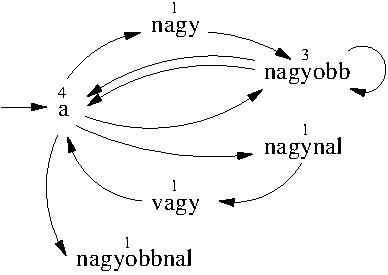
\includegraphics[width=.6\columnwidth]{img/nagyobb_nagyobb.pdf}
              \caption{,,A nagyobb nagyobb a nagynál vagy a nagy nagyobb a nagyobbnál.''
              példamondat ábrázolása.
              A dupla nyilat ábrázolhatjuk egy 2-es súllyal bíró szimpla nyíllal is.}
              \label{fig:scfr_pelda}
              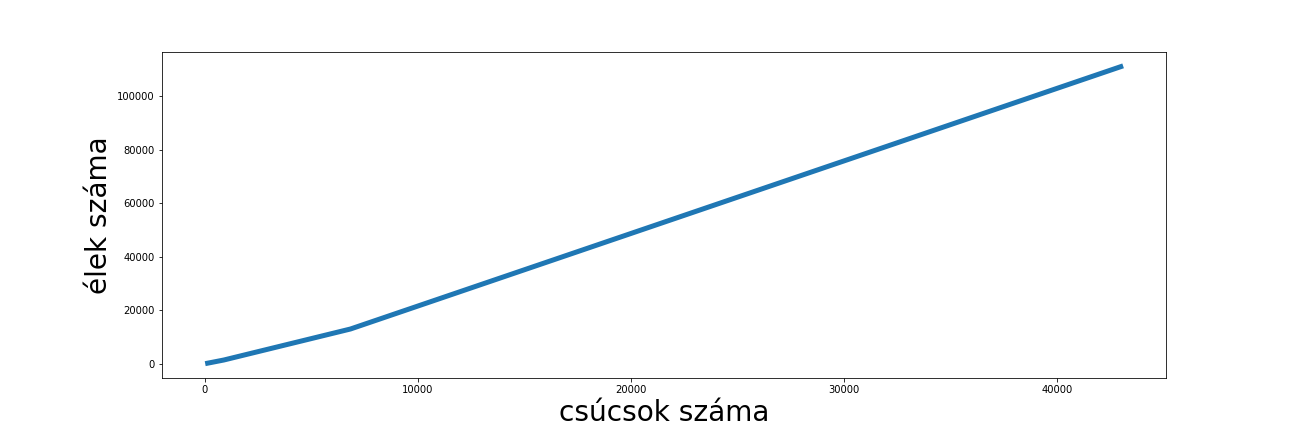
\includegraphics[width=\columnwidth]{img/nedge_vs_nnode}
          \end{figure}
        \end{block}

        %\smallskip

        \bigskip

        \begin{block}{Irányított kisvilág globálisan és\dots}%, tranzitivitás} 
          \begin{figure} 
            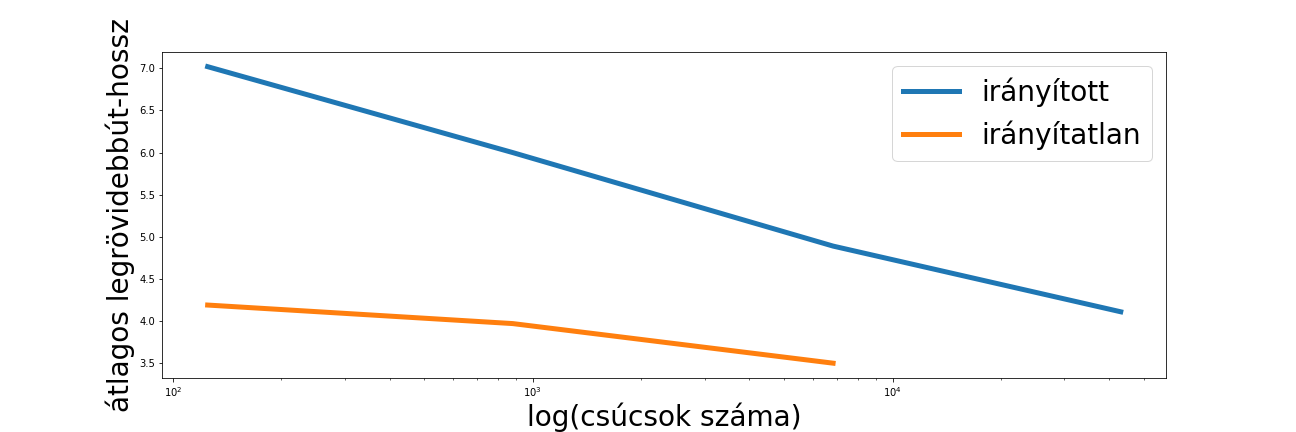
\includegraphics[width=\columnwidth]{img/avg-shortest-path-length}

            % \begin{tabular}{rrrrrrr}
            % %TODO L, tranz: kell irányítatlan?
            % \toprule
            % mondat & szókincs & bigram & \multicolumn{2}{c}{$L$} & \multicolumn{2}{c}{tranzitivitás} \\
            % &&&$\rightarrow$&--&$\rightarrow$&--\\
            % \midrule
            % 10	& 125	& 165	& 7.02	& 4.19	& 0.007463	& 0.02086 \\
            % 100	& 880	& 1343	& 6.00	& 3.97	& 0.004343	& 0.008146 \\
            % 1k  &6828	& 12952	& 4.89	& 3.50	& 0.00263	& 0.004051 \\
            % 10k & 42992	& 111141	& 4.11	& 0.001713 \\
            % 100k	& 225481	& 865512 \\
            % 1m	& 1043583	& 6082 \\
            % 10m	& 4444502	& 38167 \\
            % 47m	& 11245533	& 119857 \\
            % \bottomrule
            % \end{tabular}
          \end{figure}
        \end{block}

        \bigskip

        \begin{block}{\dots lokálisan}
          \begin{figure}
            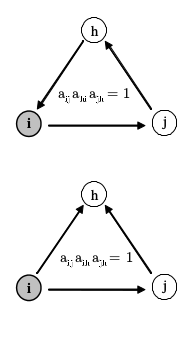
\includegraphics[width=7.5cm]{img/triangle-directions_1}
                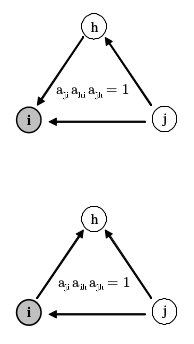
\includegraphics[width=7.5cm]{img/triangle-directions_2} 
                \caption{Irányított klaszterezési együttható \citep{fagiolo2007clustering}}

              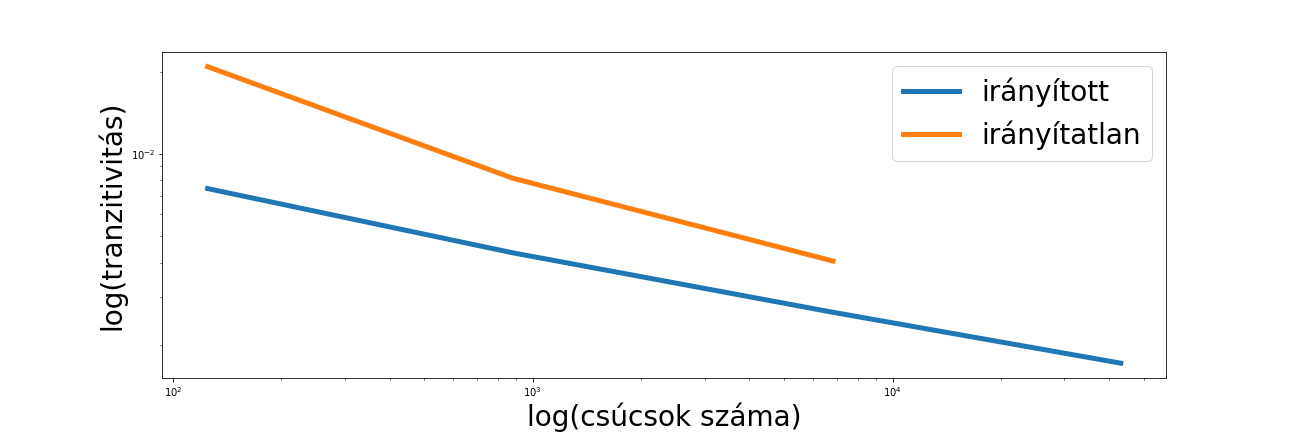
\includegraphics[width=\columnwidth]{img/trans}
          \end{figure}
        \end{block}
      \end{column}

    \begin{column}{\sepwid} \end{column}   % empty spacer column

      %%%%%%%%%%%%%%%%%%%%%%%%%%%%
      \begin{column}{\twocolwid} % középső oszlop
        %%%%%%%%%%%%%%%%%%%%%%%%%%%%

        \begin{columns} % fölső blokkok
          \begin{column}{\onecolwid}

            \begin{block}{Különcség (\emph{eccentricity})}
              \begin{itemize}
                \item egy $v$ csúcs $e_v$ \emph{különcsége} 
                  a $v$-ból az összes többi csúcsba vezető legrövidebb utak
                        hosszának maximuma
              \end{itemize}
              \begin{table}
                \begin{tabular}{ccccccc}
                  \toprule
                      mondat & \multicolumn{2}{c}{sugár, $r$} &
                      \multicolumn{2}{c}{átmérő, $d$} &
                      center  & periféria \\   
                      & \multicolumn{2}{c}{$\min e_v$} & \multicolumn{2}{c}{$\max_v
                      e_v$} & $\{v\mid e_v=r\}$ & $\{v\mid e_v=d\}$\\ 
                      & $\rightarrow$ & -- & $\rightarrow$ & -- \\
                      \midrule
                      100 & 11 & 7 & 23 & 13 & \{\texttt ., \texttt !, \texttt ?\} &
                      \{nádcukorból\}\\
                      1k  &  9 &   & 19 &    & \{\texttt ,\} & \{Megadható, two\}\\
                      \bottomrule 
                \end{tabular}
              \end{table} 
            \end{block}
          \end{column} 

    \begin{column}{\sepwid} \end{column}   % empty spacer column

          \begin{column}{\onecolwid}
            \begin{block}{Kapcsolódó irodalom}
              \begin{itemize}
                \item TextRank \citep{mihalcea2004textrank}, kulcsszókinyerés
                  \begin{quote}
                    results [...] are worse than results obtained with undirected
                          graphs, which suggests that [...] there is no natural “direction”
                  \end{quote}
                \item szemantikus hálók \citep{steyvers2005large}
                \item trigram \citep{cancho2001thesmall}
                \item a skálafüggetlen-hipe kritikája
                  \citep{willinger2009mathematics}
              \end{itemize}
            \end{block}
          \end{column}
        \end{columns}


        %%%%%%%%%%%%%%%%%%%%%%%%%%%%%%%%%%
        % Közép közép
        %%%%%%%%%%%%%%%%%%%%%%%%%%%%%%%%%% 

                \bigskip

                  \begin{block}%{Kísérletek}
                    {Közelségi központiság (\emph{closeness centrality}),
                    irányítatlan} 
                    \begin{figure}[h]
                      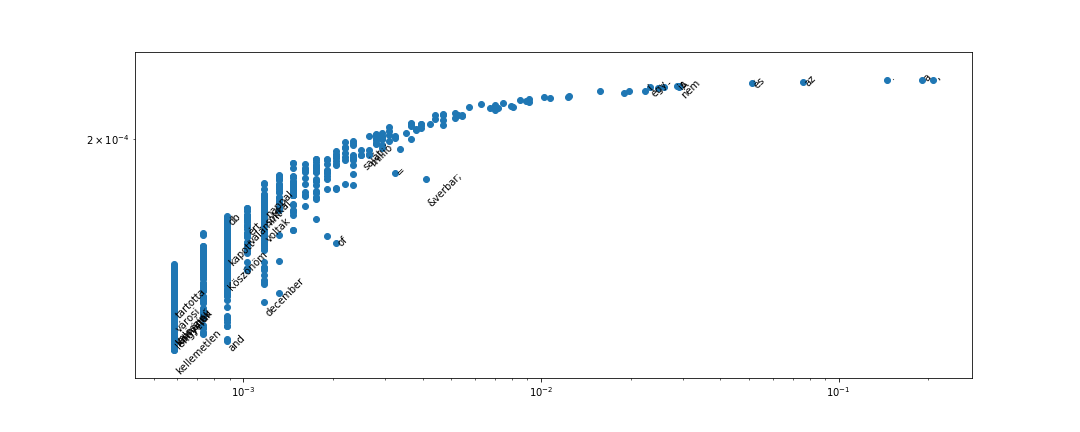
\includegraphics[width=.7\columnwidth]{img/current-flow-closeness.png}
                      \caption{%A szavak eloszlása \emph{closeness centrality} szerint.}
                        A szavak egységes eloszlásban helyezkednek el.
                      Az eloszlásból néhány olyan elem lóg ki, amely
                      ,,nem illeszkedik a magyar szövegbe'':
                      ilyen az egyenlőségjel és egy HTML entity ({\tt \&verbar;}),
                      illetve két angol szó (a \liex{the} és az \liex{of}),
                      melyek előfordulnak a korpuszban.
                      %
                      % Ez egy fokszám vs closeness_centrality grafikon, ugye?
                      Ezeknek a tokeneknek tehát kisebb
                      a közelségi központiság értékük annál,
                      mint amit gyakoriságuk alapján várnánk.
                      %
                      A kilógó elemek pontos karakterizálásához további vizsgálat szükséges.
                      }

                      \label{fig:closeness}
                    \end{figure}
                    \end{block}

        \bigskip

        \begin{block}{HITS, hyperlinkindukált témakeresés
          \emph{(Hyperlink-Induced Topic Search)}}
          \begin{columns}
            \begin{column}{\onecolwid}
              \resizebox{\columnwidth}{!}{
              \begin{tabular}{lll}
                \toprule
                & pl. & miért fontos \\
                \midrule
                hub & \href{https://index.hu/}{index.hu},
                \href{https://vajdasag.lap.hu/}{vajdasag.lap.hu} & linkek \\
                tekintély \emph{(authority)} &
                \url{http://www.nytud.hu/oszt/korpusz/} & tartalom \\
                \bottomrule
              \end{tabular}
            }
          \begin{columns}
            \begin{column}{.5\columnwidth}
              \begin{itemize}
                \item kölcsönös definíció
                  % jó hub egy olyan oldal, amely sok tekintélyes oldalra
                  % mutat, nagy tekintélyük pedig azoknak az oldalaknak van
                  % ebben a modellben, melyekre számos jó hub mutat.
                \item számítása iteríatíve 
                  \begin{itemize}
                    \item tetszőleges inicializáció
                    \item  majd minden iterációban $\rightarrow$
                  \end{itemize} \end{itemize} 
              \end{column}
            \begin{column}{.5\columnwidth}
                      \begin{align*}
                        h(v_1) &= \sum \{ a(v_2)\mid \langle v_1,v_2\rangle \in E \} \\
                        u(v_2) &= \sum \{ a(v_1)\mid \langle v_1,v_2\rangle \in E \} \\
                        u\quad &{\text{\texttt{/=}}} \sum_v u(v)^2 \\
                        a\quad &{\text{\texttt{/=}}} \sum_v a(v)^2
                      \end{align*}
            \end{column}
            \end{columns}
            \end{column}

            \begin{column}{\onecolwid} 
              \begin{figure}[h]
                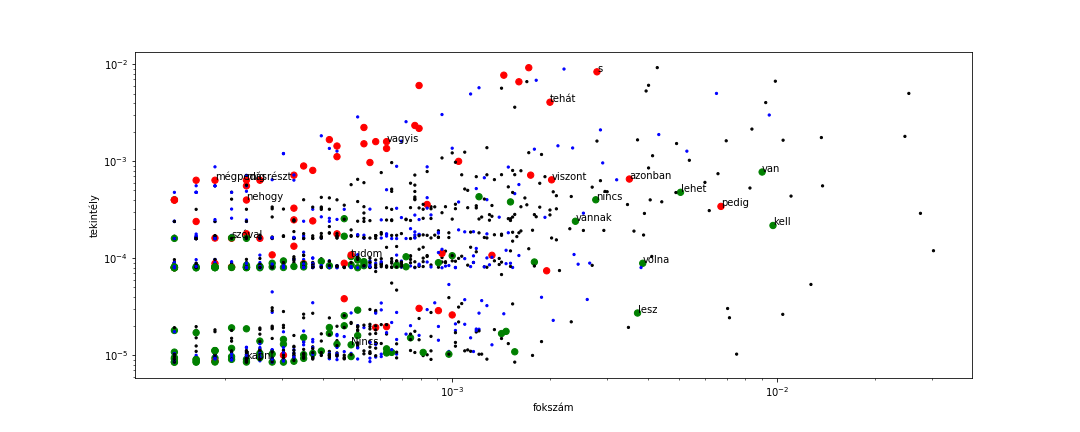
\includegraphics[width=\columnwidth]{img/conj-verb-auth.png}
                    \caption{%A HITS algoritmus eredménye.
                      A nagyobb, piros ponttal jelölt kötőszavak balra fent (magasabb
                    authority), a nagyobb, zöld ponttal jelölt igék jobbra lent (alacsonyabb
                    authority) helyezkednek el a fokszám (gyakoriság) vs authority
                    grafikonon.} 
              \end{figure}
            \end{column}
            
    \begin{column}{\sepwid} \end{column}   % empty spacer column

          \end{columns} 
              \begin{figure}
                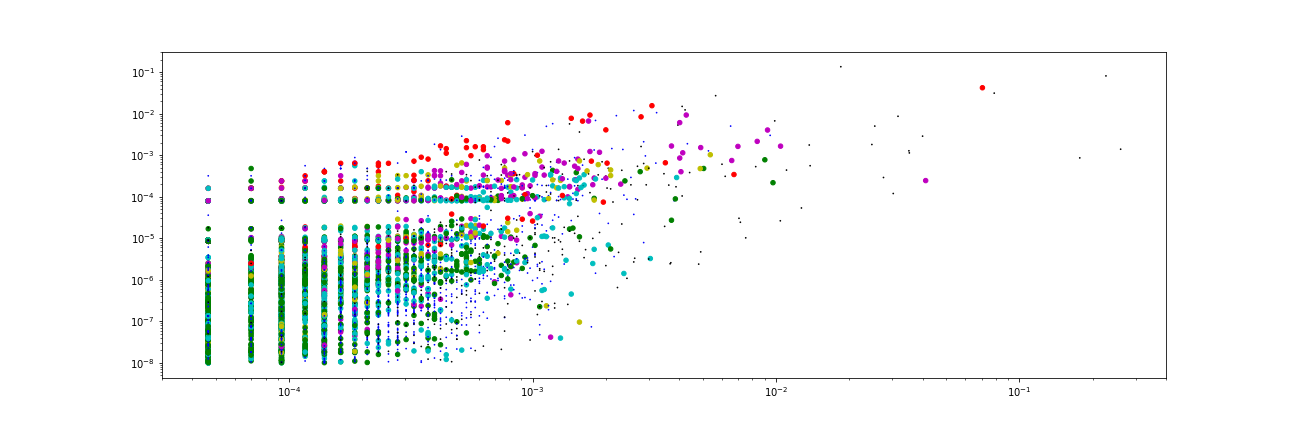
\includegraphics[width=.7\columnwidth]{img/auth_poster}
                \caption{Tekintély szófajok szerint: 
                \textcolor{red}{kötőszók},
                \textcolor{green}{igék},
                \textcolor{magenta}{határozók},
                \textcolor{cyan}{melléknevek}, és
            \textcolor{darkgoldenrod}{számnevek}.
            10 K mondat, csak a $>10^{-8}$ tekintélyű szavakat ábrázoltuk.

            }
                  \label{fig:hits-auth} 
          \end{figure}
        \end{block}

        %%%%%%%%%%%%%%%%%
      \begin{columns} % alsó blokkok
        %%%%%%%%%%%%%%%%%
        \begin{column}{\onecolwid}
          \bigskip

        \end{column}
        %\begin{column}{\onecolwid} \end{column}
      \end{columns}

    \end{column}

    \begin{column}{\sepwid} \end{column}   % empty spacer column

      %%%%%%%%%%%%%%%%%%%%%%%%%%%%
      \begin{column}{\onecolwid} % jobb oszlop
        %%%%%%%%%%%%%%%%%%%%%%%%%%%%

        \begin{block}{Központiság}
          \begin{figure}
            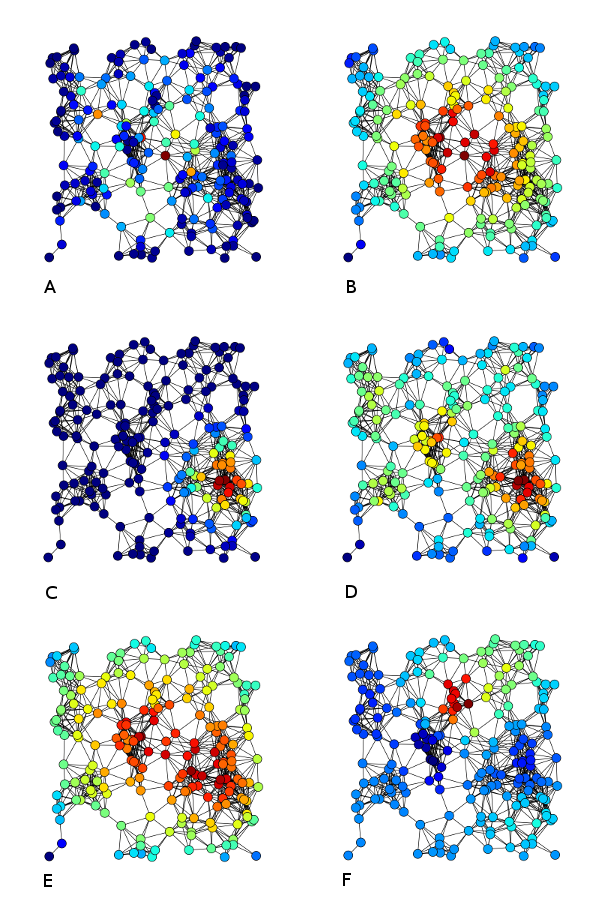
\includegraphics{img/6_centrality_measures}

              \begin{tabular}{ll}
                \alert{A} köztiség (betweenness)	& \alert{B} közelség (closeness) \\
                \alert{C} sajátvektor-	& \alert{D} fok (itt gyakoriság)\\
                \alert{E} harmonikus	& \alert{F} Katz \\
              \end{tabular}
          \end{figure}
        \end{block}

        \bigskip

        \begin{block}{További kutatás}
          \begin{itemize}
            \item klaszterek szófajok szerint?
            \item az élsúlyok skálázása távolságként
            \item irányított gráfok hatékony implementációja
            \item szemantika
              %\item még
              %\item még
              %\item még
          \end{itemize}
        \end{block}

        \bigskip

        \begin{block}{Hivatkozások}
          \small
          %\footnotesize
            \bibliographystyle{abbrvnat}
            \bibliography{minden}
        \end{block}

      \end{column} 
  \end{columns}
\end{frame}
\end{document}
